\documentclass[a4paper]{article}
\usepackage[vietnamese]{babel}
\usepackage[left=3.5cm,right=2.5cm,top=2cm,bottom=2cm]{geometry} 
\setlength{\parindent}{0pt}
\usepackage{graphicx} 
%\usepackage{wallpaper}
%\usepackage[firstpage]{draftwatermark} 
\usepackage{xcolor}
\usepackage{tikz} 
\usepackage{scrextend}
\changefontsizes{14pt}
%\usepackage{background}
\usetikzlibrary{calc}
%\backgroundsetup{scale = 1, angle = 0, opacity = 0.2,
%contents = {\includegraphics[width = 0.9\paperwidth,
%height = 0.9\paperheight, keepaspectratio] {hust.png}}}

%\backgroundsetup{scale = 1, angle = 0, opacity = 0.2,
%contents = {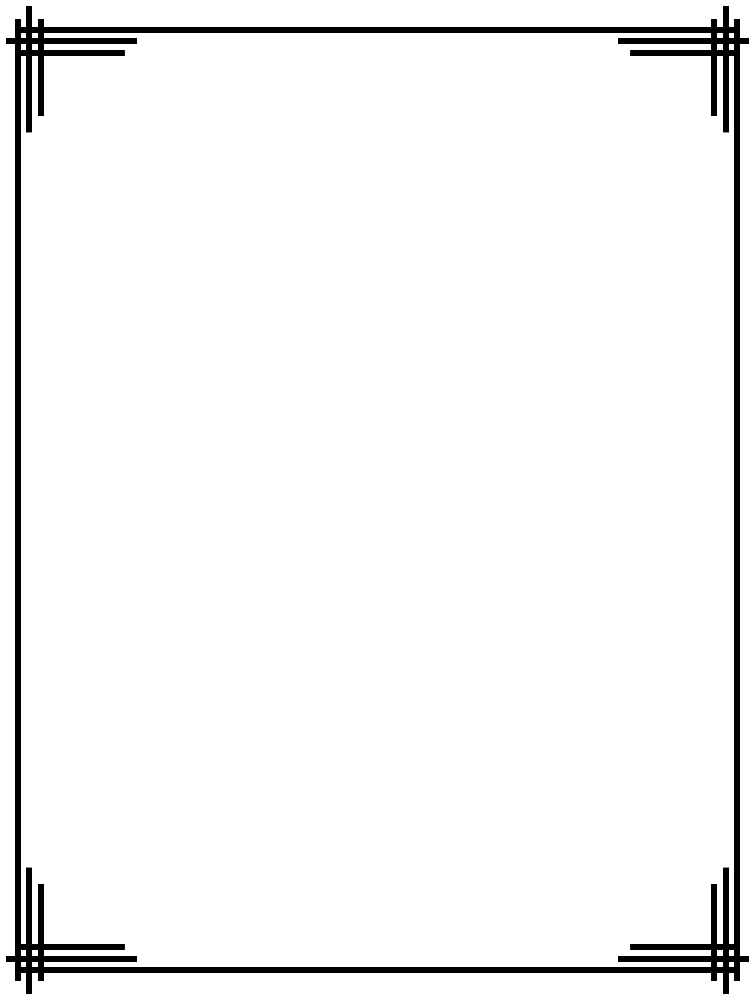
\includegraphics[width = 0.97\paperwidth,
%height = 0.97\paperheight, keepaspectratio] {bia.png}}}
\begin{document}
\begin{titlepage}
%\SetWatermarkText{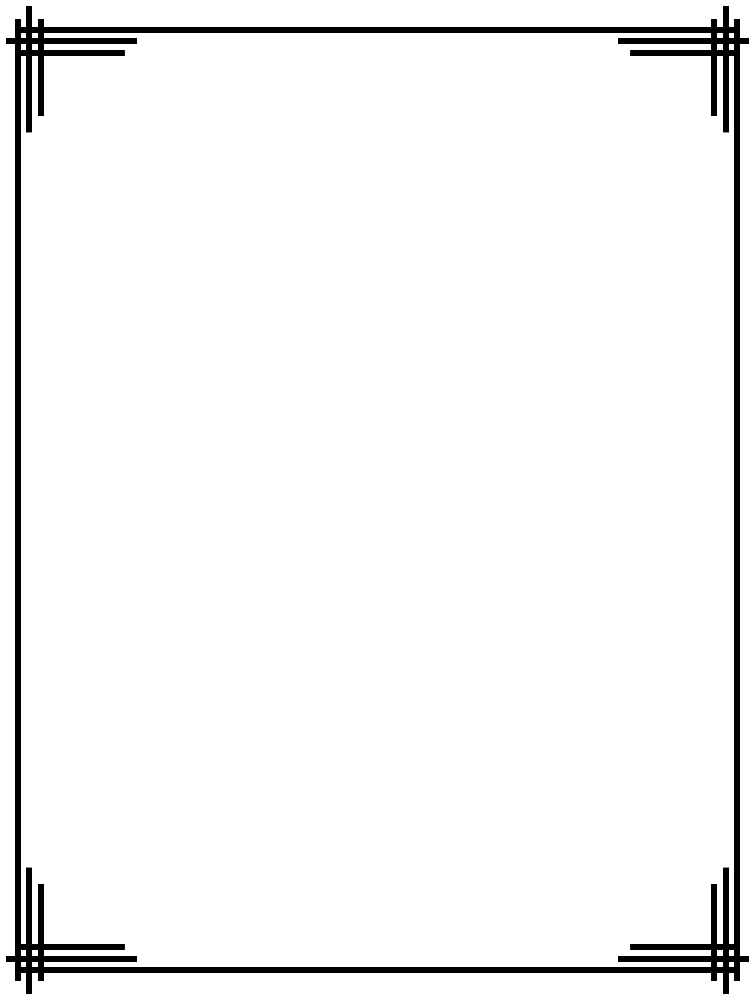
\includegraphics[width = 0.97\paperwidth,
%height = 0.97\paperheight]{bia.png}}
%\SetWatermarkAngle{0} 
%\SetWatermarkText{\includegraphics[scale=1]{hust.png}}
%\SetWatermarkAngle{0} 
\begin{tikzpicture}[remember picture,overlay,inner sep=0,outer sep=0]
     \draw[blue!70!black,line width=4pt] ([xshift=-1.5cm,yshift=-2cm]current page.north east) coordinate (A)--([xshift=1.5cm,yshift=-2cm]current page.north west) coordinate(B)--([xshift=1.5cm,yshift=2cm]current page.south west) coordinate (C)--([xshift=-1.5cm,yshift=2cm]current page.south east) coordinate(D)--cycle;

     \draw ([yshift=0.5cm,xshift=-0.5cm]A)-- ([yshift=0.5cm,xshift=0.5cm]B)--
     ([yshift=-0.5cm,xshift=0.5cm]B) --([yshift=-0.5cm,xshift=-0.5cm]B)--([yshift=0.5cm,xshift=-0.5cm]C)--([yshift=0.5cm,xshift=0.5cm]C)--([yshift=-0.5cm,xshift=0.5cm]C)-- ([yshift=-0.5cm,xshift=-0.5cm]D)--([yshift=0.5cm,xshift=-0.5cm]D)--([yshift=0.5cm,xshift=0.5cm]D)--([yshift=-0.5cm,xshift=0.5cm]A)--([yshift=-0.5cm,xshift=-0.5cm]A)--([yshift=0.5cm,xshift=-0.5cm]A);


     \draw ([yshift=-0.3cm,xshift=0.3cm]A)-- ([yshift=-0.3cm,xshift=-0.3cm]B)--
     ([yshift=0.3cm,xshift=-0.3cm]B) --([yshift=0.3cm,xshift=0.3cm]B)--([yshift=-0.3cm,xshift=0.3cm]C)--([yshift=-0.3cm,xshift=-0.3cm]C)--([yshift=0.3cm,xshift=-0.3cm]C)-- ([yshift=0.3cm,xshift=0.3cm]D)--([yshift=-0.3cm,xshift=0.3cm]D)--([yshift=-0.3cm,xshift=-0.3cm]D)--([yshift=0.3cm,xshift=-0.3cm]A)--([yshift=0.3cm,xshift=0.3cm]A)--([yshift=-0.3cm,xshift=0.3cm]A);

   \end{tikzpicture}
\begin{center}
    \vspace{10pt}
    
    \textbf{TRƯỜNG ĐẠI HỌC BÁCH KHOA TP. HỒ CHÍ MINH}
    
    \vspace{10pt}
    \textbf{KHOA KHOA HỌC ỨNG DỤNG}\\
    \vspace{10pt}
    \textbf{BỘ MÔN LÝ LUẬN CHÍNH TRỊ}\\
    \textbf{--------------------  *  ---------------------}\\[0.5cm]
\end{center}
\vspace{10pt}
\begin{center}
    
\includegraphics[scale=0.3]{LogoBK.jpg}
    
    \vspace{10pt}
    \fontsize{16pt}{15pt}\selectfont 
    \textbf{BÀI TẬP LỚN}\\
    \vspace{7pt}
    \textbf{MÔN HỌC: KINH TẾ CHÍNH TRỊ MÁC - LÊNIN}\\
    \vspace{7pt}
    \textbf{HỌC KỲ: HK231}\\[1.5cm]
\end{center}
\begin{flushleft}
    \fontsize{14pt}{17pt}\selectfont  
    \textbf{\textsl{CHỦ ĐỀ 5:}}
\end{flushleft}
\begin{center}
    \fontsize{18pt}{17pt}\selectfont 
    \textbf{\textrm{PHÁT TRIỂN CÔNG NGHỆ TRÍ THÔNG MINH NHÂN TẠO (AI) TRONG QUÁ TRÌNH CÔNG NGHIỆP HOÁ, HIỆN ĐẠI HOÁ Ở VIỆT NAM}}
\end{center}

\vspace{15pt}
\textbf{GV hướng dẫn: NGUYỄN TRUNG HIẾU}

\vspace{10pt}
\textbf{Nhóm sinh viên thực hiện: mã nhóm do gv tạo}

\begin{tabbing}
\hspace{8cm}\=\hspace{3cm}\=\hspace{3cm} \kill
{\it \textbf{Họ và tên}}\>{\it \textbf{MSSV}}\>{\it \textbf{Ghi chú}}\\
\begin{bfseries}Nguyễn Văn A \end{bfseries}\> \begin{bfseries}12345678\end{bfseries}\> \begin{bfseries}108113\end{bfseries}\\
\begin{bfseries}Nguyễn Văn A\end{bfseries}\> \begin{bfseries}12345678\end{bfseries}\> \begin{bfseries}108113\end{bfseries}\\
\begin{bfseries}Nguyễn Văn A\end{bfseries}\> \begin{bfseries}12345678\end{bfseries}\> \begin{bfseries}108113\end{bfseries}\\
\begin{bfseries}Nguyễn Văn A\end{bfseries}\> \begin{bfseries}12345678\end{bfseries}\> \begin{bfseries}108113\end{bfseries}\\
\begin{bfseries}Nguyễn Văn A\end{bfseries}\> \begin{bfseries}12345678\end{bfseries}\> \begin{bfseries}108113\end{bfseries}\\

\end{tabbing}
\vspace{10pt}
\begin{center}
    \textbf{TP.HỒ CHÍ MINH, TH.9-11/2023}
\end{center}
\end{titlepage}
\end{document}
